\documentclass[11pt]{article}

\usepackage[a4paper,margin=25mm]{geometry}
\usepackage{amsmath,amssymb}
\usepackage{booktabs}
\usepackage{graphicx}
\usepackage{hyperref}

\hypersetup{
  colorlinks=true,
  linkcolor=blue,
  citecolor=blue,
  urlcolor=blue
}

\graphicspath{{figures/}}

\title{Digital Abelian Logical Phase Control in a Correlated-Hopping Ladder}
\author{Fabien POLLY\\
\href{https://github.com/infinition/antler}{github.com/infinition/antler}}
\date{20 July 2026}

\begin{document}
\maketitle

\begin{abstract}
We report an exact-diagonalization study of a digital logical phase primitive
in a number-conserving correlated-hopping ladder. The model is a hard-core
two-leg Su-Schrieffer-Heeger ladder with a fixed rung-major Jordan-Wigner
string convention. A sequential exchange protocol is read out interferometrically
in a dressed two-state logical frame, using matched exchange and round-trip
controls at opposite statistical angles. We reconstruct the complete logical
matrix, including its singular values, leakage and off-diagonal mixing. At
$L=14$ and $N=2$, all fine-step data at $D=4,6,8,10,12$ and
$\Delta t=0.125$ follow
$\Delta\phi/\theta=-1+0.66493D^{-2.28624}$ with $R^2=0.999983$.
The retained points have worst-case leakage below $5\times10^{-5}$ and
$\sigma_{\min}>0.999975$. Registered digital path deformations give logical
unitary changes below $5.41\times10^{-5}$ at the tested operating point.
Repeated cycles remain near the same logical $Z$ axis through $n=8$.
The current gate family commutes. This work establishes an Abelian digital
phase primitive for the specified Hamiltonian; it does not demonstrate
non-Abelian braiding, universality, fault tolerance or a physical anyon
platform.
\end{abstract}

\section{Introduction}

Topological quantum computation requires a protected fusion space and
physical operations that act noncommutatively on that space
\cite{nayak2008nonabelian,kitaev2001unpaired,alicea2011wire}. A diagonal
logical phase is not sufficient. Nevertheless, a controlled Abelian primitive
is a useful intermediate result when its Hamiltonian, encoding, propagation
error and claim boundary are all explicit.

Occupation-dependent hopping provides a controlled route to one-dimensional
models with tunable statistical phases \cite{keilmann2011statistics}. In a
number-conserving setting, edge and parity structure can be subtle: a
number-conserving parent can exhibit Majorana-like properties without being a
mean-field Bogoliubov-de Gennes model \cite{iemini2015localized}. These
observations motivate the present numerical study, but neither establishes a
non-Abelian operation for the ladder studied here.

The objective of this work is narrow. We test whether a frozen,
number-conserving correlated-hopping ladder supports a reproducible digital
logical phase with a controlled deep-trap limit. The tests are designed to
separate physical localization in trap depth $D$ from numerical convergence in
the integration step $\Delta t$. We also measure path deformations,
multi-cycle composition and the commutativity of the resulting gate family.

The project name ANTLER stands for \emph{Anyonic Numerical Transport for
Logical Exchange and Robustness}. It labels the research program and its
numerical diagnostics; it does not assert that the present ladder realizes
physical anyons or non-Abelian braiding.

\section{Model and logical protocol}

\subsection{Correlated-hopping ladder}

There are $L$ rungs and two hard-core modes per rung. The rung-major site
index is $k=2j+\sigma$, with rung $j=0,\ldots,L-1$ and rail
$\sigma\in\{0,1\}$. The fixed Jordan-Wigner convention is
\begin{equation}
 a_k=\exp\!\left(i\theta\sum_{m<k}n_m\right)b_k,
 \qquad n_m=b_m^\dagger b_m .
\end{equation}
For $k<l$, the exact-diagonalization Hamiltonian in the fixed-$N$ sector is
\begin{equation}
 H(t)=-\sum_{k<l}J_{kl}\left[
 b_k^\dagger \exp\!\left(i\theta\sum_{k<m<l}n_m\right)b_l
 +\mathrm{h.c.}\right]+\sum_k\mu_k(t)n_k .
 \label{eq:hamiltonian}
\end{equation}
The rung couplings are $J_\perp=0.1$. Along either rail, the alternating
Su-Schrieffer-Heeger couplings are $J_1=0.4$ and $J_2=1.0$. The statistical
angle in Eq.~\eqref{eq:hamiltonian} is a property of this fixed correlated-
hopping convention. It is not claimed to define convention-independent
anyon statistics.

The endpoint Hamiltonian contains deep left and right edge traps. Its two
selected low-energy states are rotated into a maximally localized dressed
logical frame $\{\lvert 0_L\rangle,\lvert 1_L\rangle\}$ associated with the
left and right edge configurations. This is a logical reference frame for
control and readout. It is not asserted to be a topologically protected code.

\subsection{Sequential digital exchange}

One logical branch is mobile while the other remains trapped as a spectator.
The mobile branch is carried outward, transferred by two non-simultaneous
handoffs, and returned on the opposite rail. A matched round trip omits the
rail exchange. The two protocols have identical endpoint Hamiltonians and are
compared at $+\theta$ and $-\theta$. Figure~\ref{fig:protocol} shows the
sequence schematically.

\begin{figure}[t]
  \centering
  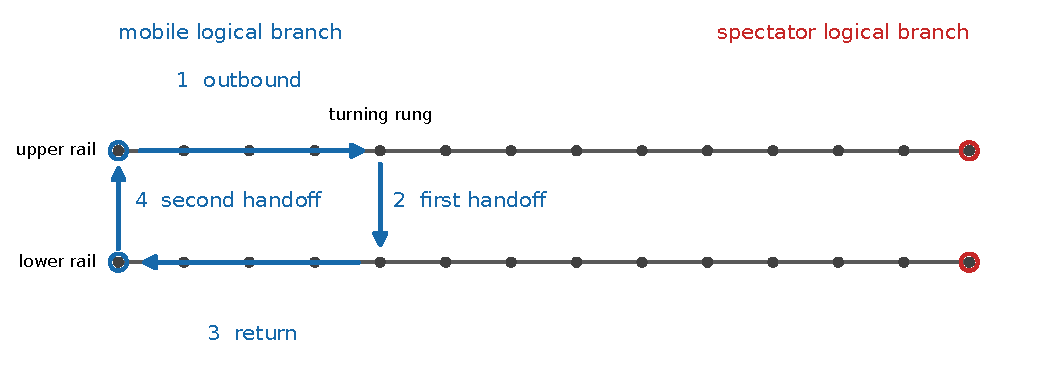
\includegraphics[width=\linewidth]{protocol_schematic.pdf}
  \caption{Ordered control sequence for the sequential protocol. The blue
  arrows show outward transport, the first rail handoff, return transport and
  the second handoff. The red edge branch is the spectator logical reference.
  The drawing is a protocol schematic, not a claim of physical particle
  worldlines in two dimensions.}
  \label{fig:protocol}
\end{figure}

For an isolated handoff, the local two-state Hamiltonian may be written as
\begin{equation}
 H_\varphi(t)=
 \begin{pmatrix}
 \epsilon_1(t) & -J\exp(i\varphi)\\
 -J\exp(-i\varphi) & \epsilon_2(t)
 \end{pmatrix}.
 \label{eq:handoff}
\end{equation}
It obeys $H_\varphi=G_\varphi H_0G_\varphi^\dagger$ with
$G_\varphi=\mathrm{diag}(\exp(i\varphi),1)$. If the avoided crossing remains
open and the handoff is adiabatic, the source state is transferred to the
target with an oriented factor $\exp(-i\varphi)$ up to a common phase. In the
strictly localized limit of the implemented sequence, one longitudinal
transfer crosses the occupied intermediate mode and contributes
$\Delta\phi=-\theta$; the matched round trip cancels its forward and reverse
contributions.

At finite trap depth, virtual configurations outside the localized handoff
subspace correct the phase, amplitude and leakage. The numerical test is thus
\begin{equation}
 \frac{\Delta\phi}{\theta}=-1+aD^{-p}+O(D^{-p-1}),
 \label{eq:fit}
\end{equation}
with the adiabatic duration scaled as $T(D)=T_\mathrm{ref}(D/D_\mathrm{ref})^2$.

\section{Numerical method and diagnostics}

All results use exact diagonalization at $L=14$ and $N=2$. The digital
propagator uses a symmetric split step: half of the diagonal trap potential,
the exactly exponentiated hopping matrix, then the second potential half
step. For each signed angle and for exchange and round-trip protocols, the
projected logical map is
\begin{equation}
 S=U_0^\dagger U(T)U_0,
\end{equation}
where $U_0$ is the endpoint logical frame. Its polar unitary is used for
logical phases, while the singular values of $S$ retain loss information.

Even-in-$\theta$ contributions are removed by combining the matched exchange
and round-trip unitaries at opposite angles. The resulting odd map is
diagonalized only after the full $2\times2$ logical reconstruction. The
reported diagnostics are the odd phase slope $\Delta\phi/\theta$, worst-case
leakage $1-\sigma_{\min}^2$, the minimum singular value, off-diagonal norm,
and the overlap-tracked isolation gap between the two selected logical
branches and the remaining spectrum during the handoffs.

The deep-limit campaign uses $\theta=0.3$, $D=4,6,8,10,12$,
$T_\mathrm{ref}=20000$, $D_\mathrm{ref}=4$ and $\Delta t=0.125$. Independent
time-step data at $D=6$ and $D=8$ use $\Delta t=0.5,0.25,0.125$. The
finite-depth path campaign uses $D=8$, $T=80000$ and $\Delta t=0.25$.
The composition campaign uses $D=6$, $T=45000$, $\Delta t=0.25$ and
$n=1,2,4,8$ cycles.

\section{Results}

\subsection{Deep-trap and time-step closure}

The five all-fine-step depth points are given in Table~\ref{tab:deep-limit}.
A fit to Eq.~\eqref{eq:fit} with the limiting value fixed to $-1$ gives
\begin{equation}
 a=0.66493,\qquad p=2.28624\pm0.00764,\qquad R^2=0.999983 .
\end{equation}
The residual root-mean-square error is $3.91\times10^{-5}$. All five retained
points have leakage below $5\times10^{-5}$ and a positive sampled handoff
isolation gap. Figure~\ref{fig:deep} displays both the finite-depth correction
and the approach to the fixed digital limit.

\begin{figure}[t]
  \centering
  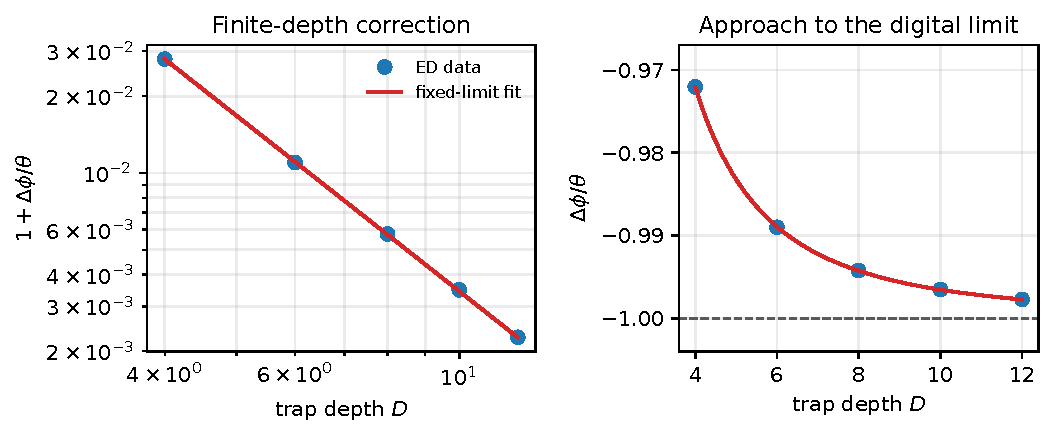
\includegraphics[width=\linewidth]{deep_limit.pdf}
  \caption{All-fine-step deep-limit data. Left: the correction
  $1+\Delta\phi/\theta$ on logarithmic axes. Right: the raw slope and the
  fixed limiting value $-1$. The curve is a two-parameter fit, not an
  independently derived exponent.}
  \label{fig:deep}
\end{figure}

The time-step study is reported in Table~\ref{tab:timestep}. At both
$D=6$ and $D=8$, the coarse $\Delta t=0.5$ rows exhibit substantial leakage
and are explicit numerical failures. Reducing to $\Delta t=0.25$ restores
the intended gate, while the $\Delta t=0.125$ rows have leakage near
$10^{-5}$. Thus the depth trend used in Fig.~\ref{fig:deep} is not inferred
from the coarse integrator.

\subsection{Protocol deformations and composition}

Eleven registered deformations preserve the sequential protocol and endpoint
Hamiltonian while varying ramp profile, handoff duration, pauses, trap
depths, separation or handoff order. The largest phase shift from the
baseline is $7.65\times10^{-5}$ radians and the largest relative logical-unitary
distance is $5.41\times10^{-5}$ at the tested operating point
(Table~\ref{tab:path} and Fig.~\ref{fig:path}). This is finite-depth protocol
robustness, not a standalone proof of topological protection.

\begin{figure}[t]
  \centering
  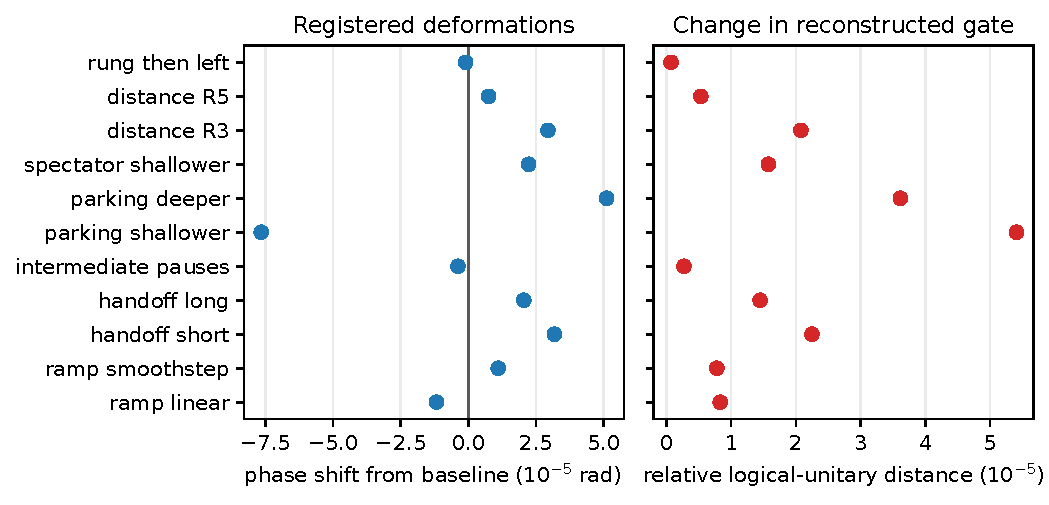
\includegraphics[width=\linewidth]{path_invariance.pdf}
  \caption{Effect of the ten non-baseline protocol deformations. Left: odd
  phase shift relative to the baseline. Right: distance between reconstructed
  logical unitaries after removal of the common global phase.}
  \label{fig:path}
\end{figure}

For repeated cycles, the phase additivity error reaches $2.57\times10^{-2}$
radians at $n=8$. This residual is reported rather than absorbed in phase
unwrapping. The worst-case leakage remains between $2.12\times10^{-4}$ and
$2.46\times10^{-4}$ over the four tested values of $n$, and the rotation axis
remains close to $Z$ (Table~\ref{tab:composition} and Fig.~\ref{fig:composition}).
There is no observed superlinear leakage signature within this four-point
test, but this does not establish a long-depth fault model.

\begin{figure}[t]
  \centering
  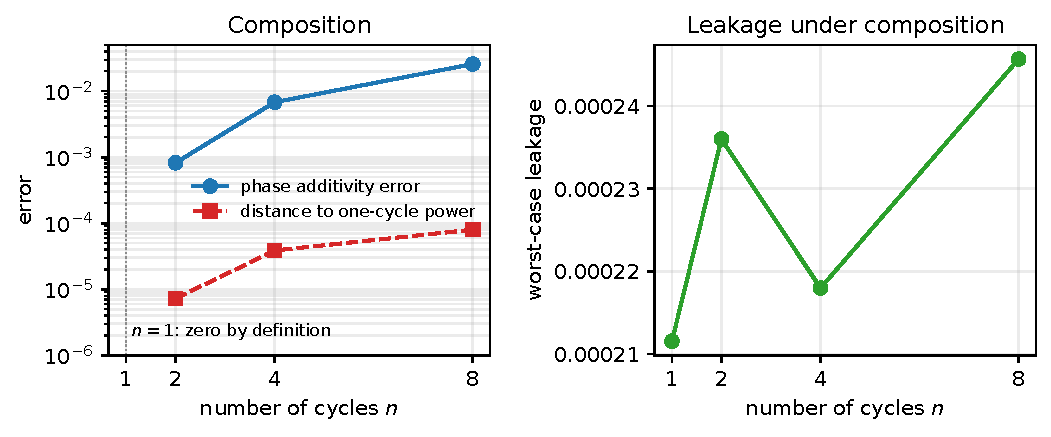
\includegraphics[width=\linewidth]{composition.pdf}
  \caption{Repeated-cycle composition. The one-cycle phase-additivity error is
  identically zero and is not placed on the logarithmic axis. Leakage remains
  small over the tested range, while the finite coherent phase error grows
  with cycle count.}
  \label{fig:composition}
\end{figure}

% Generated by paper/generate_figures.py. Do not edit by hand.
\begin{table}[t]
\centering
\caption{Fine-step deep-limit data at $\theta=0.3$ and $\Delta t=0.125$. The protocol duration follows $T(D)=20000(D/4)^2$.}
\label{tab:deep-limit}
\begin{tabular}{rrrrrr}
\toprule
$D$ & $T$ & $\Delta\phi/\theta$ & leakage & $\sigma_{\min}$ & handoff gap \\
\midrule
4 & 20000 & -0.972041 & 3.02e-05 & 0.999985 & 6.68e-04 \\
6 & 45000 & -0.989005 & 1.14e-05 & 0.999994 & 5.30e-03 \\
8 & 80000 & -0.994233 & 2.25e-05 & 0.999989 & 4.43e-03 \\
10 & 125000 & -0.996517 & 3.42e-05 & 0.999983 & 1.27e-04 \\
12 & 180000 & -0.997730 & 4.97e-05 & 0.999975 & 8.76e-03 \\
\bottomrule
\end{tabular}
\end{table}

\begin{table}[t]
\centering
\caption{Independent time-step check. The $\Delta t=0.5$ rows are retained as a resolved coarse-step failure, rather than being used in the closure fit.}
\label{tab:timestep}
\begin{tabular}{rrrrr}
\toprule
$D$ & $\Delta t$ & $\Delta\phi/\theta$ & leakage & $\sigma_{\min}$ \\
\midrule
6 & 0.500 & -0.926576 & 4.20e-01 & 0.761595 \\
6 & 0.250 & -0.990352 & 2.12e-04 & 0.999894 \\
6 & 0.125 & -0.989005 & 1.14e-05 & 0.999994 \\
8 & 0.500 & 3.392471 & 9.99e-01 & 0.028334 \\
8 & 0.250 & -0.995348 & 4.71e-04 & 0.999765 \\
8 & 0.125 & -0.994233 & 2.25e-05 & 0.999989 \\
\bottomrule
\end{tabular}
\end{table}

\begin{table}[t]
\centering
\caption{Repeated-cycle composition at $D=6$, $\theta=0.3$ and $\Delta t=0.25$.}
\label{tab:composition}
\begin{tabular}{rrrrr}
\toprule
$n$ & phase error (rad) & leakage & one-cycle-power distance & $Z$-axis drift \\
\midrule
1 & 0.000e+00 & 2.12e-04 & 3.14e-16 & 1.50e-07 \\
2 & 8.232e-04 & 2.36e-04 & 7.24e-06 & 8.01e-08 \\
4 & 6.809e-03 & 2.18e-04 & 3.87e-05 & 1.97e-07 \\
8 & 2.574e-02 & 2.46e-04 & 8.01e-05 & 2.38e-08 \\
\bottomrule
\end{tabular}
\end{table}

\begin{table}[t]
\centering
\caption{Summary of the eleven finite-depth protocol deformations at $D=8$, $\theta=0.3$ and $\Delta t=0.25$.}
\label{tab:path}
\begin{tabular}{lr}
\toprule
quantity & maximum value \\
\midrule
largest phase shift & 7.648e-05 \\
largest logical-unitary distance & 5.408e-05 \\
largest error to $-\theta$ & 1.447e-03 \\
\bottomrule
\end{tabular}
\end{table}


\subsection{Commutativity}

The reconstructed gates are effectively diagonal $Z$ rotations. An earlier
three-angle audit gave commutator norms of $4.49\times10^{-7}$,
$5.32\times10^{-7}$ and $2.89\times10^{-7}$ for angle pairs
$(0.3,0.6)$, $(0.3,0.9)$ and $(0.6,0.9)$, respectively. These values are
numerical residuals around the expected commuting family, not evidence of a
second logical generator. The present operation therefore cannot by itself
realize a non-Abelian braid or a universal gate set.

\section{Discussion and claim boundary}

The main result is a reproducible digital Abelian phase primitive for the
Hamiltonian in Eq.~\eqref{eq:hamiltonian}. The finite-depth sequence agrees
with the localized two-level transfer rule, and the independent time-step
study separates physical trap-depth convergence from a coarse-step artifact.
The full logical reconstruction is important here: phase alone would not
detect the failures at $\Delta t=0.5$ or quantify the retained leakage.

Several boundaries are essential. First, the Jordan-Wigner string is fixed by
the rung-major representation and the result is tied to that correlated-
hopping model. Second, the calculation is an exact-diagonalization result at
$L=14$, $N=2$; it is not a thermodynamic-limit or experimental robustness
certificate. Third, finite path deformations and near-diagonal composition do
not make the gate topological. Finally, a family satisfying
\begin{equation}
 [U_Z(\theta_1),U_Z(\theta_2)]=0
\end{equation}
cannot supply the noncommuting exchanges required for a non-Abelian braid.

The next research question is therefore not whether to relabel this operation
as a braid. It is whether a microscopic extension can supply a locally
protected fusion space and two derived exchanges with a nonzero commutator.
That question requires separate evidence for locality, a protected code space,
physical control terms and a non-Abelian algebra.

\section{Conclusion}

The ANTLER ladder supports a numerically closed Abelian digital logical phase
primitive in the registered $L=14$, $N=2$ protocol. The fine-step depth scan
approaches $\Delta\phi=-\theta$ with a quantified finite-depth correction,
and the associated controls bound leakage, numerical resolution, finite-depth
deformations and short repeated-cycle behavior. The results do not establish
non-Abelian statistics or topological quantum computation. They provide a
reproducible baseline against which any future non-Abelian extension must be
tested.

\section*{Data and code availability}

All scripts, numerical JSON files, figure-generation code and the logical
closure check are available at
\href{https://github.com/infinition/antler}{github.com/infinition/antler}.
The public repository includes the Phase 0 to 4.7 reproducibility archive.

\bibliographystyle{unsrt}
\bibliography{references}

\end{document}
